\documentclass{article}
\usepackage{fancyhdr}
\usepackage{extramarks}
\usepackage{parskip}
\usepackage{setspace}
\usepackage{graphicx}
\usepackage{url}
\usepackage[hidelinks]{hyperref}
\usepackage{listings}
\usepackage{color}

\graphicspath{ {images/} }
\topmargin=-0.45in
\evensidemargin=0in
\oddsidemargin=0in
\textwidth=6.5in
\textheight=9.0in
\headsep=0.25in

\linespread{1.1}

\pagestyle{fancy}
\lhead{CreateGraphics Project}
\rhead{Javascript/Grace}
\lfoot{\lastxmark}
\cfoot{\thepage}

\renewcommand\headrulewidth{0.4pt}
\renewcommand\footrulewidth{0.4pt}

\setlength\parindent{0pt}

\definecolor{dkgreen}{rgb}{0,0.6,0}
\definecolor{gray}{rgb}{0.5,0.5,0.5}
\definecolor{mauve}{rgb}{0.58,0,0.82}

\lstset{frame=tb,
  language=Java,
  aboveskip=3mm,
  belowskip=3mm,
  showstringspaces=false,
  columns=flexible,
  basicstyle={\small\ttfamily},
  numbers=none,
  numberstyle=\tiny\color{gray},
  keywordstyle=\color{blue},
  commentstyle=\color{dkgreen},
  stringstyle=\color{mauve},
  breaklines=true,
  breakatwhitespace=true,
  tabsize=3
}

\begin{document}

{\raggedleft Kristina Frye, Konstantin Macarenco, Tyler Poole \par}
{\raggedleft CS 420/520 \par}
{\raggedleft June 8, 2015 \par}
{\raggedleft Final Project \par} 

\section {Introduction}
The CreateGraphics is a graphics package for Grace designed as a replacement for the 
existing ObjectDraw. It is based upon the Open Source Createjs Javascript project that can be found
at \url{http://www.createjs.com/}. Createjs is a rich graphics library with a lot of functionality. This
project only implements its most basic functionality and can be considered a proof of concept
more than anything. However, we are confident that the framework that we have created
could be easily expanded to include more of the Createjs functionality.

\section {Architecture}
There are two major pieces to the CreateGraphics library: createJsGraphicsWrapper and
createGraphics.

createJsGraphicsWrapper provides short methods that wrap corresponding Createjs Javascript
methods and objects into Grace objects. The objects in this file create an interface for
the Javascript methods with as much one-to-one correspondence between Grace and 
Javascript as possible in order to maintain as much functionality and flexibility as possible.

createGraphics is a Grace-only file consisting of objects and methods that call the
createJsGraphicsWrapper. The idea was the build a nice Grace interface that will 
work with the more technical wrapper functions.

See Figure \ref{fig:layers} for a depiction of the different layers involved in the CreateGraphics
library. The ``user program'' at the top refers to the code that the programmer will create
in order to place graphics into the graphics window.

\begin{figure}[h]
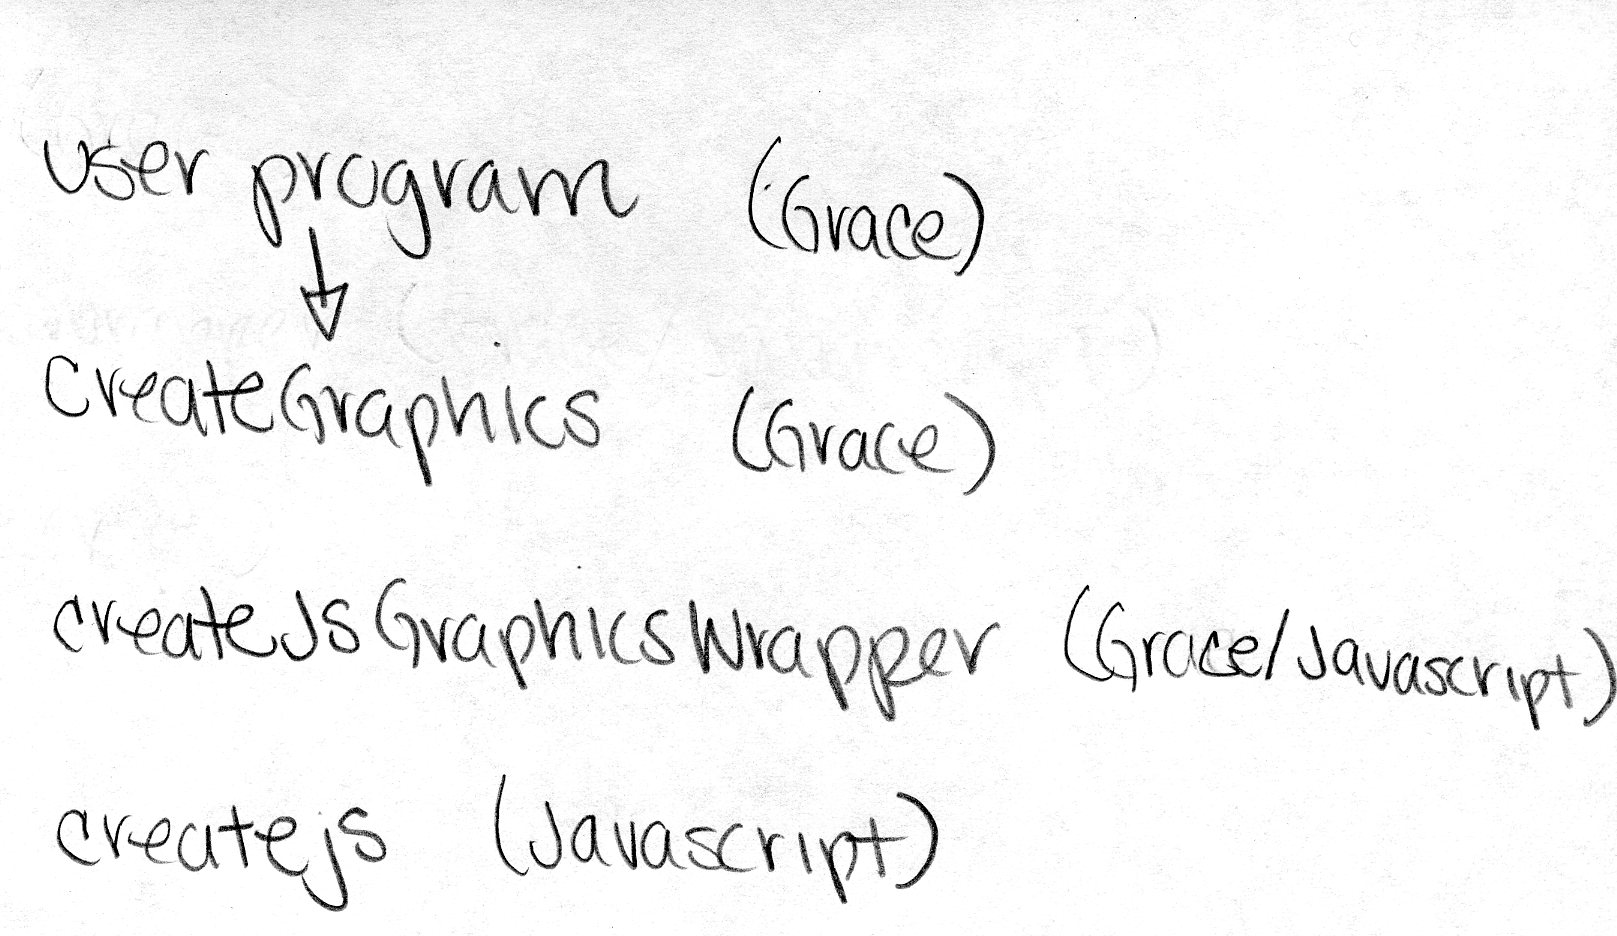
\includegraphics[scale=0.5]{layers}
\centering
\caption{createGraphics layers}
\label{fig:layers}
\end{figure}

\subsection{createJsGraphicsWrapper}
The createJsGraphicsWrapper file (see Figure \ref{fig:createjsGraphicsWrapper}) consists of a number of related objects that contain
javascript native code that calls the Createjs javascript library.

Stage is the Createjs version of the HTML canvas with additional functionality. It holds
all the the shape objects.

CommonGraphics is a base object that contains the functionality common to both the
shape and container objects such as location, bounds, and moving.

Shape is the base shape object. It inherits CommonGraphics. It contains functionality
that is common to all shape objects.

Container is a holding object that can be used to place multiple shape objects together.
For instance, you could use a container to create a button holding rectangle and text
objects.

The individual shape objects are also defined in this file including circle, rect, roundRect,
ellipse, polyStar, line, and customObject. Each shape has its own draw routine.

\begin{figure}
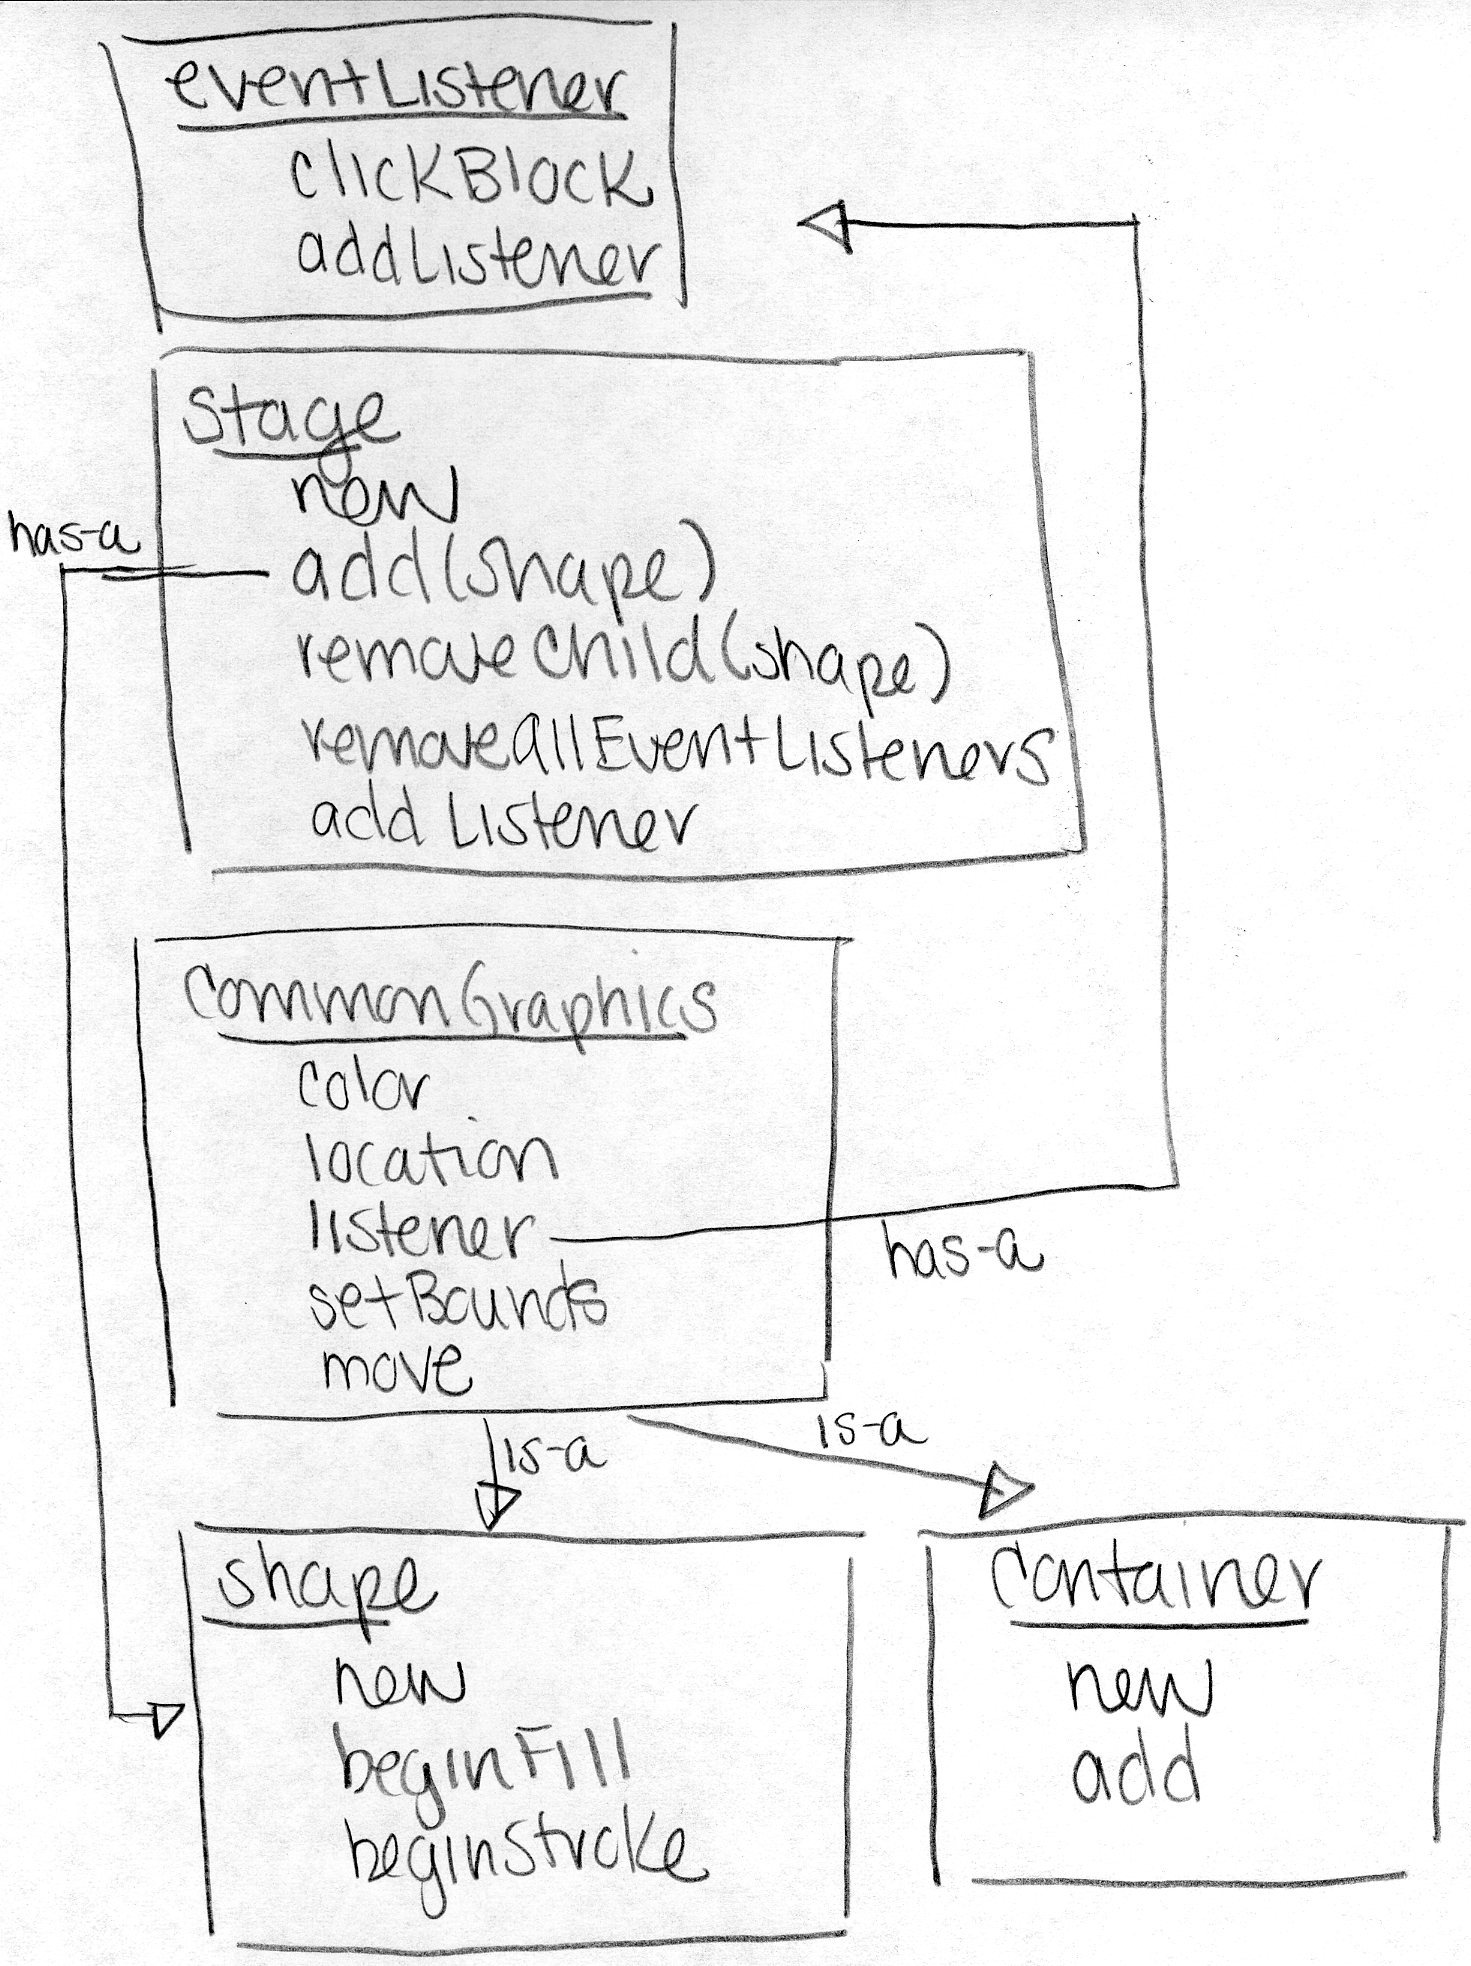
\includegraphics[scale=0.5]{createJsGraphicsWrapper}
\centering
\caption{createJsGraphicsWrapper}
\label{fig:createjsGraphicsWrapper}
\end{figure}

\subsection{createGraphics}
createGraphics.grace (see Figure \ref{fig:createGraphics}) consists of a nice interface for
programmers to use in order to create graphics. 

The parent object ``shape'' for all concrete shapes (circle, rectangle, ellipse, text, etc) is
defined here as well as the main graphics object that is used to create the window, the
canvas, and hold all reference to the created shapes.

In order to make the shapes easy to configure, most configuration variables (such as location,
color, size, etc) are public. This allows the user to set them with easy calls such as
color := ``red'' and location := 20@20. ``Chaining'' methods have also been defined in order
to combine configurations onto one line such as: circle.colored(``red'').at(20@20).draw.

Click handlers are added by simple defining a click variable with a block such as that shown 
in Figure \ref{fig:click}.
\begin{figure}[h]
\begin{lstlisting}
circle.click := { 
  print("clicked circle") 
  circle.color := "blue"
  circle.update
}
\end{lstlisting}
\caption{Click handler}
\label{fig:click}
\end{figure}

\begin{figure}
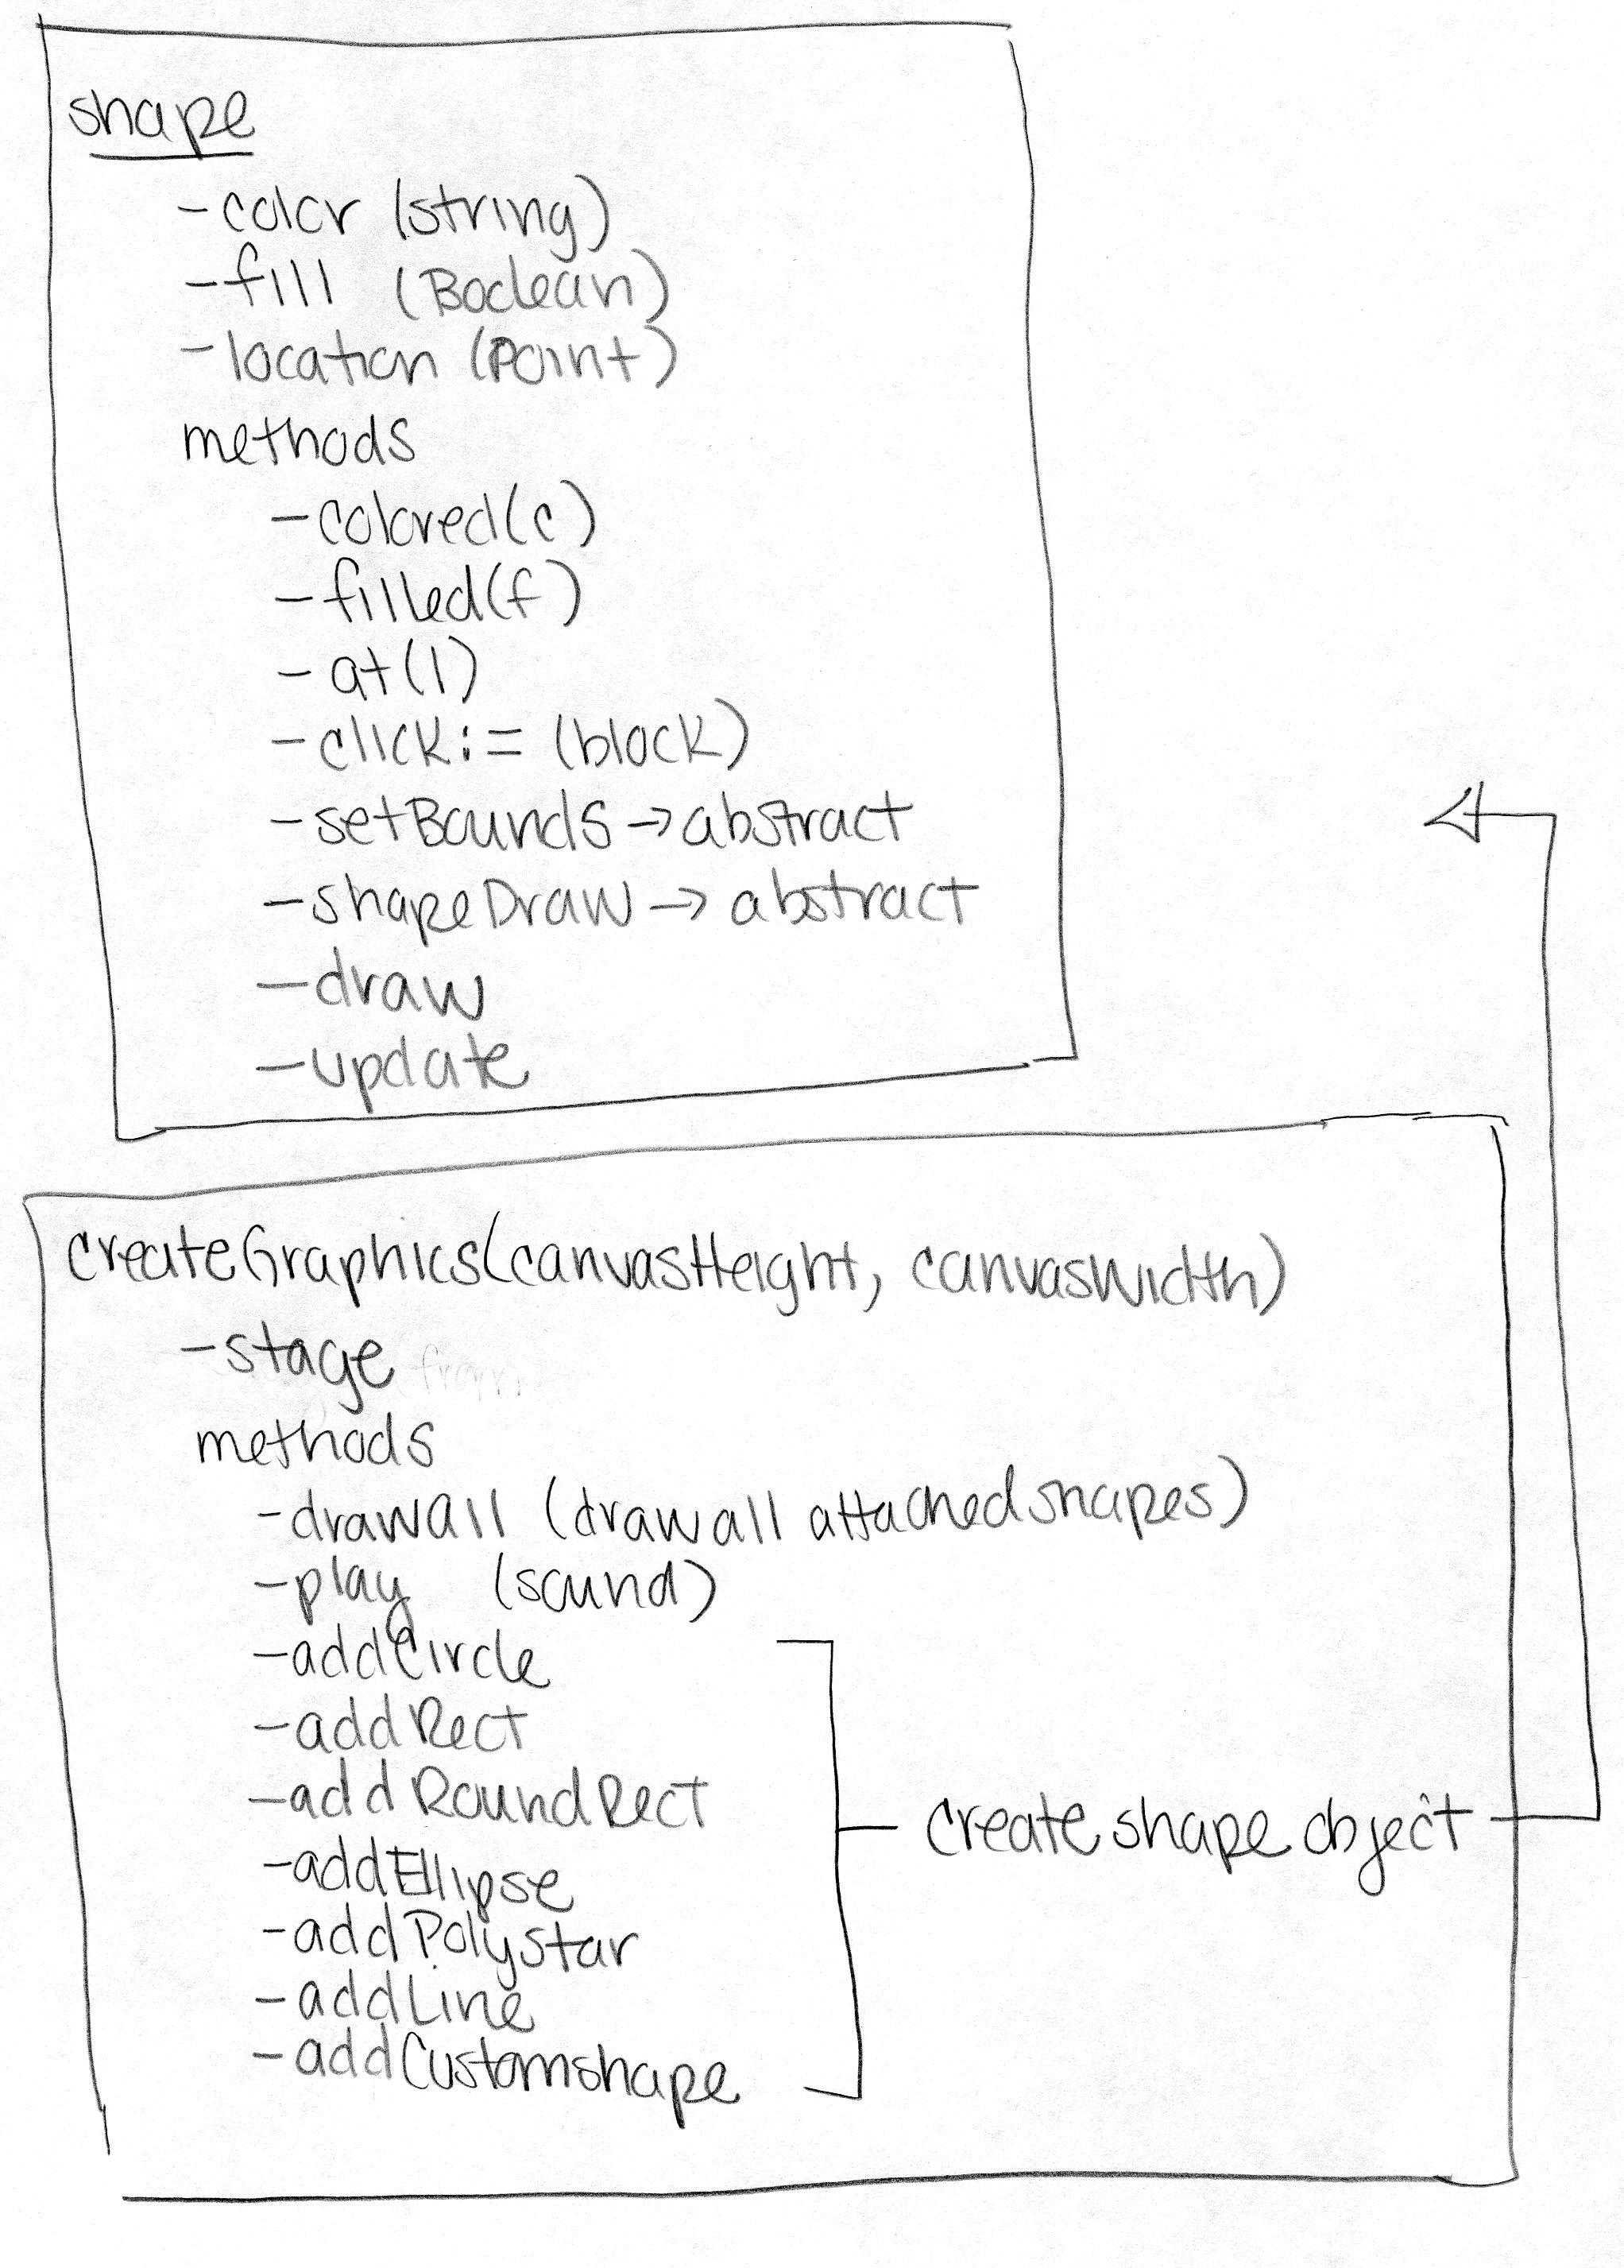
\includegraphics[scale=0.5]{createGraphics}
\centering
\caption{createGraphics}
\label{fig:createGraphics}
\end{figure}

\section{Challenges}
The biggest challenge of this project was to get the interface between the javascript Createjs library and the Grace
compiler working. In order to get the graphics working, we examined the existing ObjectDraw object to see
how it worked, figured out how the calls would work in straight Javascript, and then used the Javascript console
in the Chrome browser to step through the code and figure everything worked together. One of the complications
is that graphics are usually drawn in the main browser window. However, the goal in this case was to open a
secondary "pop-up" window and draw the graphics in that window. Since this is not the usual way that Javascript
is typically used, we ended up having to use a few workarounds.

One of these workarounds involves the event listener for the click handler. The Createjs library normally allows the
developer to assign click handlers to the individual shape objects that are created. So, if you create a circle, you can
assign a click handler directly to the circle. This handler only is activated when the circle is clicked. However, because
we are using the pop-up window, this turned out not to be possible. This appears to either be a bug or a missing
feature in Createjs, but the event listeners on individual shapes are not working when used with the pop-up window.
However, the event handler for the ``stage,'' which is the Createjs specialized version of the HTML5 canvas, does
work. So we assign all event handlers to the stage and check the mouse position in order to determine which
object was clicked. This is not as clean or efficient as adding the event handler directly to the shape, but it works. 
Another possibility in the future would be to designate part of the Grace compiler webpage for the graphics display.
This would get rid of the "pop-up" issue and would allow a much greater variety in mouse handling.

Another challenge was adding sound capability. We were hoping that we could load the sound files when the
graphics library was loaded. That way the user who is not working with the graphics library would not have to load
the sound fields into the browser every time the Grace compiler was used. However, this didn't turn out to work very
well. When loaded with the graphics library, the sound would play the first time the program loaded. However, if
we tried to run the program again, the sounds would not play unless we reloaded the entire Grace browser webpage.
Therefore we added the sound load into the main Grace index.html file, choosing only a small sampling of sounds with
a relatively small file size.

\section {Achievements}
We are proud of the resulting user interface of the createGraphics library. Although it doesn't yet have a large
number of features, we have provided a good framework that could easily be built upon, and the existing user
interface should be easy for the beginning programmer to work with. We have made it as "Gracelike" as possible
and provided default settings whenever they were needed in order to make it quick and simple to use. We think
it's going to be a good improvement on the existing graphics library once some additional functionality is added.

\end{document}